\subsection{Fermis Goldene Regel}
	Betrachte zeitlich konstante Störung
		\begin{align*}
			H^1(t) &= \underbrace{\Theta (t)}_{\substack{Heaviside}} H^1 \\
		\end{align*}
	$\Rightarrow$ für $m \neq n$, 1.Ordnung Störungstheorie:
		\begin{align*}
			P_{mn}(t) 
			&= \frac{1}{\hbar^2} \left| \braket{m | H^1 | n}\right|^2 
			\cdot \left| \int_{0}^{t} \diff t' e^{-i(\omega_m-\omega_n) t'} \right|^2 \\
			&= \frac{4}{\hbar^2} \frac{\sin^2[(\omega_m-\omega_n)
			\frac{t_0}{2}]}{(\omega_m-\omega_n)^2} 
			\left| \braket{m | H^1 | n}\right|^2
		\end{align*}
	\begin{figure*} [h]
		\begin{center}
			\includegraphics[width=10cm]{Ersatzgraph1.jpg}
		\end{center}
	\end{figure*}
		\begin{equation*}
			\lim\limits_{t \rightarrow \infty} \frac{4 \sin^2(\frac{\omega}{2} t)}{\omega^2 t} = 2 \pi \delta (\omega)
		\end{equation*}
	Annahme $\ket{m} = \ket{\alpha}$ liegt im Kontinuierlichen Teil des Spektrums von $H^0$.
	
	Beispiel H-Atom mit
		\begin{align*}
			E_n &= - \frac{1}{2} \frac{m c^2 \alpha^2}{n^2} &
			\ket{\alpha} \text{nicht normiert} \\
			E_{\alpha 0} &\leq E_\alpha \leq E_{\alpha 1}
		\end{align*}
	\begin{figure*} [h]
		\begin{center}
			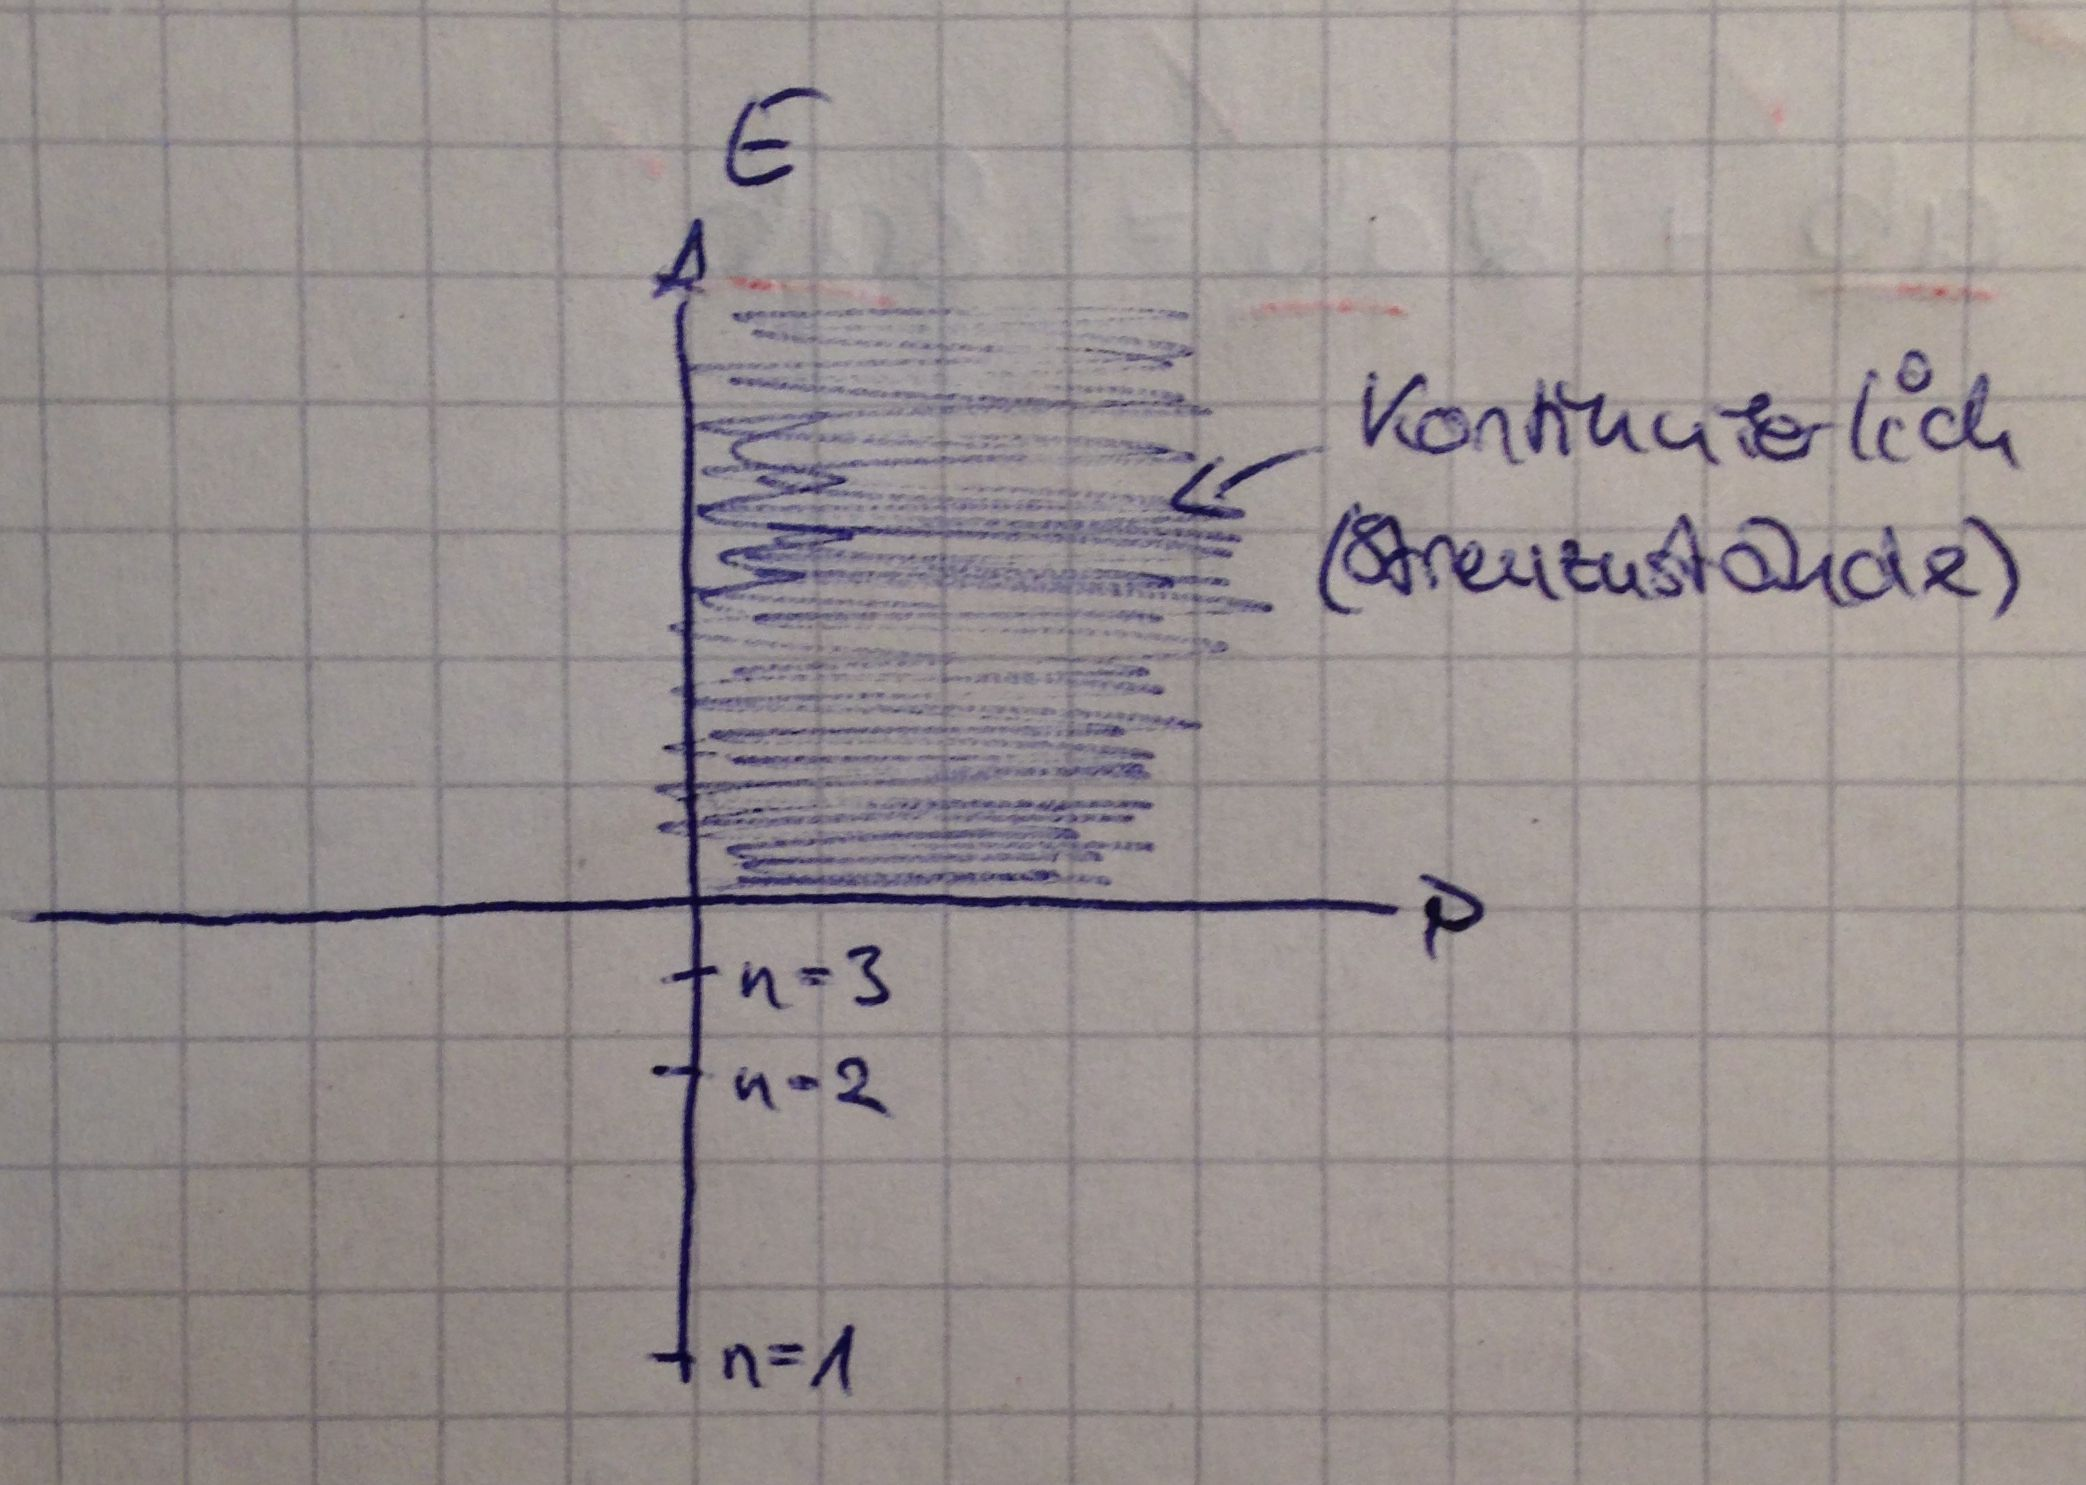
\includegraphics[width=10cm]{Ersatzgraph2.jpg}
		\end{center}
	\end{figure*}

	$P_{\alpha n}(t)$ ist Übergangswahrscheinlichkeits\underline{dichte}
	
	Übergangswahrscheinlichkeit: 
		\begin{equation*}
			\int_{\alpha_0}^{\alpha_1} \diff \alpha P_{\alpha n} (t)
		\end{equation*}
	Übergangsrate (Übergangswahrscheinlichkeit pro Zeiteinheit)
		\begin{align*}
			\underbrace{W_{\alpha \leftarrow n}}_{
				\mathclap{\text{Übergangsrate von~} n \text{~nach~} \alpha}}
			&= \int \diff \alpha \frac{P_{an}(t)}{t} \\
			&\underset{t \rightarrow \infty}{=} 
			\int \diff \alpha \frac{2 \pi}{\hbar^2} 
			\delta(\omega_\alpha - \omega_n) \left| \braket{m | H^1 | n}\right|^2 \\
			&= \int \diff \alpha \frac{2 \pi}{\hbar} 
			\delta (E_\alpha - E_n) \left| \braket{\alpha | H^1 | n}\right|^2
		\end{align*}
	(hier meinte Herr Prof. Bali mit einem Pfeil auf $E_\alpha$: Zeitunabhängige Störung erzwingt Energieerhaltung)
	
	Dichte von Zuständen:
		\begin{align*}
			\rho &= \int \diff \alpha \delta (E_\alpha - E)  \\
			\diff \alpha &= \rho(E_\alpha) \diff E_\alpha: \text{~Zahl der Zustände im ``Ìntervall''~} \diff E_\alpha
		\end{align*}
		\begin{align*}
			\boxed{
				W_{\alpha \leftarrow n} = \frac{2 \pi}{\hbar} \rho(E_n)
					\left| \braket{\alpha | H^1 | n}\right|^2
				}
			\text{~Fermis ``Goldene Regel'' (Wenzel)}
		\end{align*}
	Probleme bei 
		\begin{itemize}
			\item $t$ sehr groß $\Rightarrow \int \diff \alpha P_{\alpha n} > 1$.
			\item $t  << \frac{1}{|\omega_\alpha - \omega_n|}$ (keine $\delta$- Funktion)   
		\end{itemize}	
	Gültigkeitsbereich:
		\begin{itemize}
			\item $\Delta E$ Verteilung der Endzustände muss größer sein als die Breite von $\frac{\sin^2 (\frac{1}{2}(\omega_\alpha - \omega_n) t)}{(\omega_\alpha - \omega_n)^2}$. Damit $\delta$- Funktionsapproximation gerechtfertigt ist, muss $t \gg \frac{2 \alpha \pi}{\Delta E}$ (Version der Unschärferelation)
			\item $t$ muss klein genug sein, damit 1.Ordnung Störungstheorie gerechtfertigt ist:
			\\ $t \ll \frac{1}{W_{\alpha \leftarrow n}}$
		\end{itemize}